% !TEX root = ../main.tex

\section{The Challenge of Bayesian Inference}
\label{sec:inf:challenge}

In the previous chapter we introduced the concept of Bayesian modelling and showed how we
can combine prior information $p(\theta)$ and a likelihood model $p(\mathcal{D}|\theta)$ using Bayes' rule 
(i.e.~\eqref{eq:bayes}), to produce a posterior $p(\theta|\mathcal{D})$ on variables $\theta$ that
characterizes both our prior information and information from the data $\mathcal{D}$.  We now consider the
problem of how to calculate (or more typically approximate) this posterior, a process 
known as Bayesian \emph{inference}.
At first this may seem like a straight forward problem: by Bayes' rule we have that
$p(\theta|\mathcal{D})\propto p(\mathcal{D}|\theta)p(\theta)$ and so we already know the relative probability of any one
value of $\theta$ compared to another.  In practice, this could hardly be further from the
truth.  Bayesian inference for the general class of graphical models is in fact an 
NP-hard problem \citep{cooper1990computational,dagum1993approximating}.  We can break
it down into key challenges: calculating the normalization constant
$p(\mathcal{D}) = \int p(\mathcal{D}|\theta)p(\theta)d\theta$ and providing a useful characterization of the posterior, for
example an object we can draw samples from.  Many inference schemes, for example Markov
chain Monte Carlo (MCMC) methods \citep{hastings1970monte}, will not
try to tackle these challenges directly and instead look to generate samples directly from 
the posterior.  However, this breakdown will still prove useful in illustrating the intuitions
about the difficulties presented by Bayesian inference.

\subsection{The Normalization Constant}
\label{sec:inf:challenge:norm}

Calculating the normalization constant in Bayesian inference is essentially a problem of
integration.  Our target, $p(\mathcal{D})$, is the expectation of the likelihood under the prior,
hence the name \emph{marginal likelihood}.  When $p(\mathcal{D})$ is known, the posterior can be evaluated
exactly at any possible input point using~\eqref{eq:bayes} directly.  When it is unknown, we lack
a scaling in the evaluation of any point and so we have no concept of how relatively 
significant that point is relative to the distribution as a whole.  For example, for a discrete
problem then if we know the normalizing constant, we can evaluate the exact probability of any
particular $\theta$ by evaluating that point alone.  If we do not know the normalizing constant, we do
not know if there are other substantially more probable events that we have thus-far missed, which
would in turn imply that the queried point has a negligible chance of occurring.
 
To give a more explicit example, consider a model where $\theta \in \{1,2,3\}$ with a corresponding uniform prior $P(\theta) = 1/3$
for each $\theta$.  Now presume that for some reason that we are only able to evaluate the likelihood at 
$\theta=1$ and $\theta=2$, giving $p(\mathcal{D}|\theta=1)=1$ and $p(\mathcal{D}|\theta=2)=10$ respectively.  Depending on the marginal
likelihood $p(\mathcal{D})$, the posterior probability of $P(\theta=2 | \mathcal{D})$ will vary wildly.  For example,
$p(\mathcal{D})=4$ gives $P(\theta=2 | \mathcal{D}) = 5/6$, while $p(\mathcal{D})=1000$ gives $P(\theta=2 | \mathcal{D}) = 1/100$.  Though this
example may seem far-fetched, this is the scenario almost always seen in practice for realistic
models, at least those with non-trivial solutions.   Typically it is not
possible to enumerate all the possible values of $\theta$ in reasonable time and we are left 
wondering - how much probability mass is left that we have not seen?  The problem is even worse 
in the setting where $\theta$ is continuous, for
which it is naturally impossible to evaluate all possible values for $\theta$.  
Knowing the posterior only up to a normalization constant is deceptively unhelpful - we never
know how much of the probability mass we have missed and therefore whether the probability (or
probability density) where we have looked so far is tiny compared to some other dominant region
we are yet to explore.  At its heart, the problem of Bayesian inference is a problem
of where to concentrate our finite computational resources so that we can effectively characterize
the posterior.  If $p(\mathcal{D})$ is known, then we immediately know whether we are looking in the right
place or whether there are places left to look that we are yet to find.  This brings us onto
our second challenge -- knowing the posterior in closed form is often not enough.

\subsection{Characterizing the Posterior}
\label{sec:inf:challenge:post}

Once with have the normalization constant, it might seem that we are done; after all
we now have the exact form the posterior using in Bayes' rule.  Unfortunately, it tends to
be the case, at least when $\theta$ is continuous, that is this insufficient to carry out most
tasks that we might want to use our posterior for.  There are a number of different, often
overlapping, reasons for wanting to calculate a posterior including
\begin{itemize}
	\item To calculate the posterior probability or probability density for one or more particular
	instances of the variables.
	\item To calculate the expected value of some function, $\mu_f = \E_{p(\theta|\mathcal{D})}\left[f(\theta)\right]$.
	For example, we might want to calculate the expected values of the variables themselves
	$\mu_\theta = E_{p(\theta|\mathcal{D})} \left[\theta\right]$ as a point estimate.
	\item To make predictions.  For example, in a supervised learning task then our data typically
	comprises of a series of input output pairs $\mathcal{D} = \{x_n,y_n\}_{n=1:N}$ and we
	wish to predict the output at some new input $\tilde{x}$.  In the fully Bayesian framework, one
	does this using the \emph{posterior predictive distribution}
	\[
	p(\tilde{y} | \tilde{x}) = \int p(\tilde{y}|\tilde{x},\theta) p(\theta | \mathcal{D}) d\theta.
	\]
	Note that this is a particular case of calculating an expectation under the posterior.
	\item To find the most probable variable values $\theta^* = \argmax_{\theta} p(\theta|\mathcal{D})$.  
	This is known
	as maximum a posteriori estimation and will be discussed in Chapter~\ref{chp:opt}.
	\item To produce samples from, or form some other useful characterization of, the posterior that can
	then passed on to another part of a computational pipeline or directly observed by a user.
	\item To estimate a marginal probability distribution over some variables of particular
	interest.  For example, if $\theta=\{u,v\}$ then we might be interest in the marginal
	$p(u|\mathcal{D})$.
\end{itemize}
If $\theta$ is continuous or some elements of $\theta$ are continuous then only the first of
these can be carried out directly using the form of the posterior provided by Bayes' rule
with known normalization constant.  We, therefore, see that knowing the normalization alone
will not be enough to fully solve the Bayesian inference problem in a useful manner.  In
particular, it will generally not sufficient in order to be able to \emph{sample} from the
posterior.  As we will see later, the ability to sample will be at the core of most practical uses
for the posterior as it allows use of Monte Carlo
 methods~\citep{metropolis1949monte,robert2004monte,rubinstein2016simulation}, which
 can in turn be used to carry out many of the outlined tasks.

To further demonstrate why knowing the normalization constant is insufficient
for most Bayesian inference tasks, we consider the following a simple example
\begin{subequations}
\label{eq:inf:example}
\begin{align}
p(\theta) &= \textsc{Gamma}\left(\theta; 3, 1\right) = \frac{\theta^2 \exp(-\theta)}{2},
 \quad \theta\in\left(0,\infty\right), \\
p(y=5|\theta) &= \textsc{Student-t}\left(5-\theta;2\right) = 
\frac{\Gamma (1.5)}{\sqrt{2\pi}}\left(1+\frac{\left(y-\theta\right)^2}{2}\right)^{-3/2}, \\
p(\theta |y=5) &\approx 5.348556 \; \theta^2
	 \exp(-\theta)\left(2+(5-\theta)^2\right)^{-3/2}\label{eq:inf:example-post}.
\end{align}
\end{subequations}
Here we have that the prior on $\theta$ is distributed according to a gamma
distribution with shape parameter $3$ and scale parameter $1$.  The likelihood
function is a student-t distribution on the difference between $\theta$ and the
output $y=5$.  Using a numerical integration over $\theta$ the normalization
constant can be calculated to a high accuracy, giving the provided closed-form
equation for the posterior.  This posterior, along with the prior and likelihood are shown Figure~\ref{fig:inf:inf-example}.

\begin{figure}[t]
	\centering
	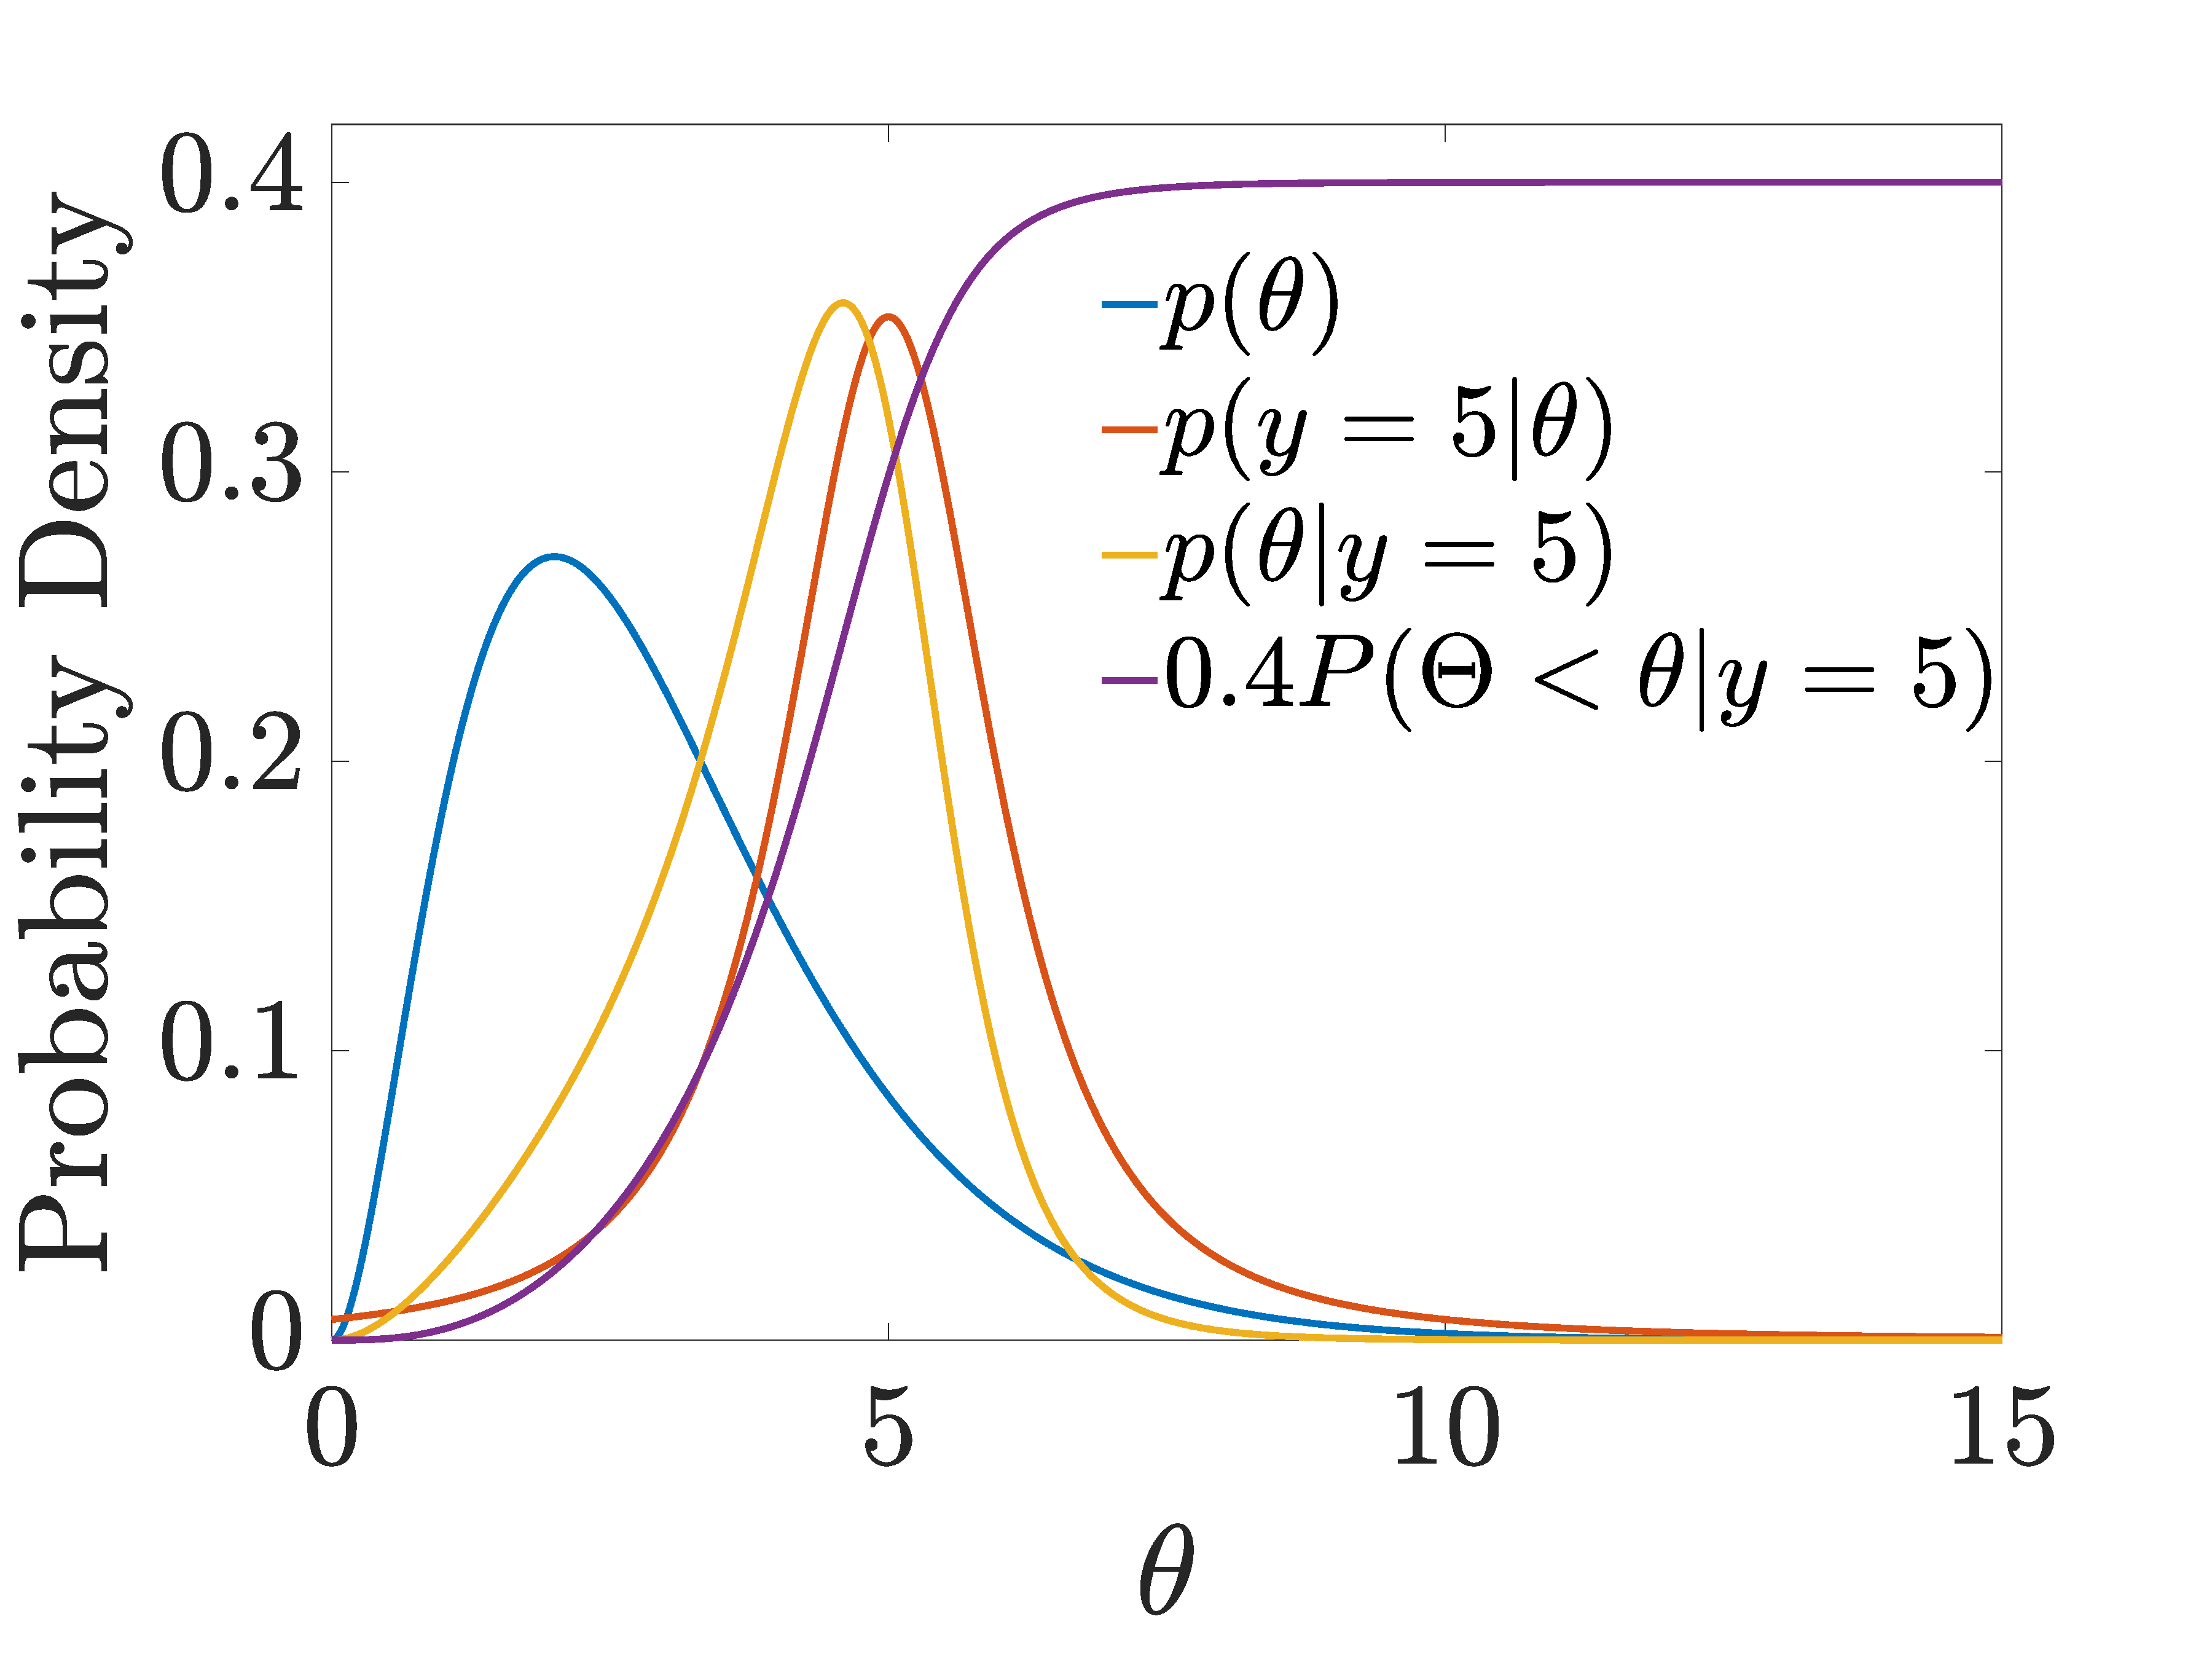
\includegraphics[width=0.65\textwidth]{inf_example}
	\caption{Example inference for problem given
		in~\eqref{eq:inf:example}. Also shown is the cumulative distribution for
		the posterior as per~\eqref{eq:inf:cum-example}.  This is scaled by a factor
		of $1/2$ for visualization.  \label{fig:inf:inf-example}}
\end{figure}

Here knowing the marginal likelihood means that we have a 
closed-form equation for the posterior.  Image though that we 
wish to sample from it.  As it does not correspond to a standard distribution,
we cannot simply call a standard sampling procedure.  There is, in fact, no way
to directly sampling from this distribution without doing further calculations.  If
we also know the inverse of the cumulative density function of the posterior
\begin{align}
\label{eq:inf:cum-example}
P(\Theta\le\theta | y=5) = \int_{\Theta=0}^{\Theta=\theta}  p(\theta=\Theta | y=5) d\Theta,
\end{align}
then we can sample from the posterior by sampling $\hat{u} \sim \textsc{Uniform}(0,1)$ and
then taking as our sample $\hat{\theta} = P^{-1}(\hat{u})$ such that 
$\hat{u} = P(\Theta\le\hat{\theta} | y=5)$.  However, the cumulative distribution function
and its inverse cannot be calculated analytically.  Though in this simple one dimensional
problem they can be easily estimated numerically, this will prove prohibitively difficult
for most problems where $\theta$ has more than a few dimensions.  Similarly, if we
wish to estimate an expectation with respect to this posterior we could do this relatively
easily numerically for this simple problem, for example using Simpson's rule, but in higher
dimensions this will be impractical.

There are a number of indirect methods we could use instead to sample from the posterior
such as rejection sampling, importance sampling, and MCMC.  However, as we will show
in the Section~\ref{sec:inf:foundation}, these all only require that we can evaluate an unnormalized version of
target distribution, such that they side-step the need to calculate the marginal 
likelihood.  Nonetheless, knowledge of the marginal likelihood can still be helpful in
a number of scenarios (e.g. in adapting our inference algorithm) for the reasons outlined in 
Section~\ref{sec:inf:challenge:norm}.